\clearpage
\section{improved TEP-Net}

blindtext

\subsection{Backbones}

\begin{table}[H]
    \centering
    \resizebox{\textwidth}{!}{
        \begin{tabular}{lcccccc}
            \hline
            \rowcolor{white} \textbf{Model} & \textbf{Parameters} & \textbf{Flops} & \textbf{MACs} & \textbf{Latency TRT FP32 / FP16} & \textbf{IoU} & \textbf{Switch Eval} \\
            \hline
            \rowcolor[gray]{0.9} TEP-ENB3   & 14.57M            &                & 4.87G          & 24.89 / 15.26 ms        & \textbf{0.9753} & 91.18 \% \\ 
            \rowcolor{white}     TEP-RN18   & 15.64M            &                & 9.48G          & 9.48 / 3.25 ms          & 0.9695          & 80.15 \% \\ 
            \hline
            \rowcolor[gray]{0.9} MNV3-Small & \textbf{5.33M}    & \textbf{1.09B} & \textbf{0.30G} & \textbf{3.13 / 2.05 ms} & 0.9619          & 73.53 \% \\ 
            \rowcolor{white}     MNV3-Large & 7.27M             & 4.3B           & 1.17G          & 6.41 / 3.75 ms          & 0.9649          &  \\ 
            \rowcolor[gray]{0.9} DN121      & 11.42M            & 59.22B         & 15.14G         & 29.53 / 16.52 ms        & 0.9750          &  \\ 
            \rowcolor{white}     DN161      & 30.9M             & 161.47B        & 40.98G         & 75.77 / 34.02 ms        & 0.9746          &  \\ 
            \rowcolor[gray]{0.9} DN169      & 16.96M            & 70.19B         & 17.95G         & 38.87 / 22.51 ms        & 0.9748          &  \\ 
            \rowcolor{white}     DN201      & 22.57M            & 89.66B         & 22.93G         & 52.14 / 29.94 ms        & 0.9751          & \textbf{93.38 \%}  \\
            \hline
        \end{tabular}
    }
    \caption{Backbone Results}
    \label{tab:backboneResults}
\end{table}

\subsection{Pooling Layers}

\begin{table}[H]
    \centering
    \hspace{-3cm}
    \begin{minipage}{0.03\textwidth} % Für den vertikal gedrehten Text
        \rotatebox{90}{\textbf{\hspace{0.5cm} Max Pool \hspace{0.5cm} Average Pool \hspace{0.8cm} No Pool \hspace{1cm}}}
    \end{minipage}%
    \resizebox{0.95\textwidth}{!}{
    \begin{minipage}{0.95\textwidth} % Für die Tabelle
        \begin{tabular}{lcccccc}
            \hline
            \rowcolor{white} \textbf{Model} & \textbf{Parameters} & \textbf{Flops} & \textbf{MACs} & \textbf{Latency TRT FP32 / FP16} & \textbf{IoU} & \textbf{Switch Eval} \\
            \hline
            \rowcolor[gray]{0.9} TEP-ENB3      & 14.57M            &                & 4.87G          & 24.89 / 15.26 ms        & \textbf{0.9753} & 91.18 \% \\ 
            \rowcolor{white}     TEP-RN18      & 15.64M            &                & 9.48G          & 9.48 / 3.25 ms          & 0.9695          & 80.15 \% \\ 
            \rowcolor[gray]{0.9} MNV3-Small    & \textbf{5.33M}    & \textbf{1.09B} & \textbf{0.30G} & \textbf{3.13 / 2.05 ms} & 0.9619          & 73.53 \% \\ 
            \rowcolor{white}     DN201         & 22.57M            & 89.66B         & 22.93G         & 52.14 / 29.94 ms        & 0.9751          & 93.38 \% \\
            \hline
            \rowcolor[gray]{0.9} TEP-ENB3-AP   & 15.35M            & 19.86B         & 5.36G          & 25.64 / 15.25 ms        & 0.9134          & 93.38 \% \\ 
            \rowcolor{white}     TEP-RN18-AP   & 16.69M            & 38.45B         & 9.8G           & 10.18 / 3.42 ms         & 0.9658          & 91.18 \% \\ 
            \rowcolor[gray]{0.9} MNV3-Small-AP & 5.53M             & 1.19B          & 0.35G          & 3.24 / 2.1 ms           & 0.9502          & 58.82 \% \\ 
            \rowcolor{white}     DN201-AP      & -                 & -              & -              & Expected to be high     & -               & - \\ 
            \hline
            \rowcolor[gray]{0.9} TEP-ENB3-MP   & 15.35M            & 19.86B         & 5.36G          & 25.68 / 15.5 ms         & 0.9730          & \textbf{94.85} \% \\ 
            \rowcolor{white}     TEP-RN18-MP   & 16.69M            & 38.45B         & 9.8G           & 9.89 / 3.41 ms          & 0.9688          & 91.91 \% \\ 
            \rowcolor[gray]{0.9} MNV3-Small-MP & 5.53M             & 1.19B          & 0.35G          & 3.25 / 2.11 ms          & 0.9595          & 68.38 \% \\ 
            \rowcolor{white}     DN201-MP      & -                 & -              & -              & Expected to be high     & -               & - \\ 
            \hline
        \end{tabular}
    \end{minipage}
    }
    \caption{Pooling Layers Results}
    \label{tab:poolongResults}
\end{table}

\subsection{Prediction Heads}

\begin{table}[H]
    \centering
    \resizebox{\textwidth}{!}{
    \begin{tabular}{lcccccc}
        \hline
        \rowcolor{white} \textbf{Model} & \textbf{Parameters} & \textbf{Flops} & \textbf{MACs} & \textbf{Latency TRT FP32 / FP16} & \textbf{IoU} & \textbf{Switch Eval} \\
        \hline
        \rowcolor[gray]{0.9} ENB3-MP      & \textbf{15.35M} & \textbf{19.86B} & \textbf{5.36G} & \textbf{25.68 / 15.5 ms}  & \textbf{0.9730} & 94.85 \% \\ 
        \hline
        \rowcolor{white}     DEPTH-HEAD   & 23.75M & 19.88B & 5.37G & 25.57 / 15.74 ms & 0.9721 & 91.91 \% \\ 
        \rowcolor[gray]{0.9} WIDTH-HEAD   & 36.59M & 19.91B & 5.38G & 26.51 / 16.09 ms & 0.9723 & 97.06 \% \\ 
        \rowcolor{white}     TRAPEZE-HEAD & 32.92M & 19.90B & 5.38G & 25.87 / 16.09 ms & 0.9715 & \textbf{97.79} \% \\ 
        \hline
    \end{tabular}
    }
    \caption{Prediction Heads Results}
    \label{tab:predHeadsResults}
\end{table}

\section{Comparison Baseline to improved Version}

\begin{figure}[H]
    \centering
    \begin{minipage}{0.2\textwidth} % Linke Seite für Text
        \centering
        \textbf{original TEP-Net}\\
        EfficientNet-B3
    \end{minipage}%
    \hfill
    \begin{minipage}{0.6\textwidth} % Mittlere Spalte für die Figure
        \centering
        % Hier die Original-Figur
        \begin{subfigure}[b]{0.48\textwidth}
            \centering
            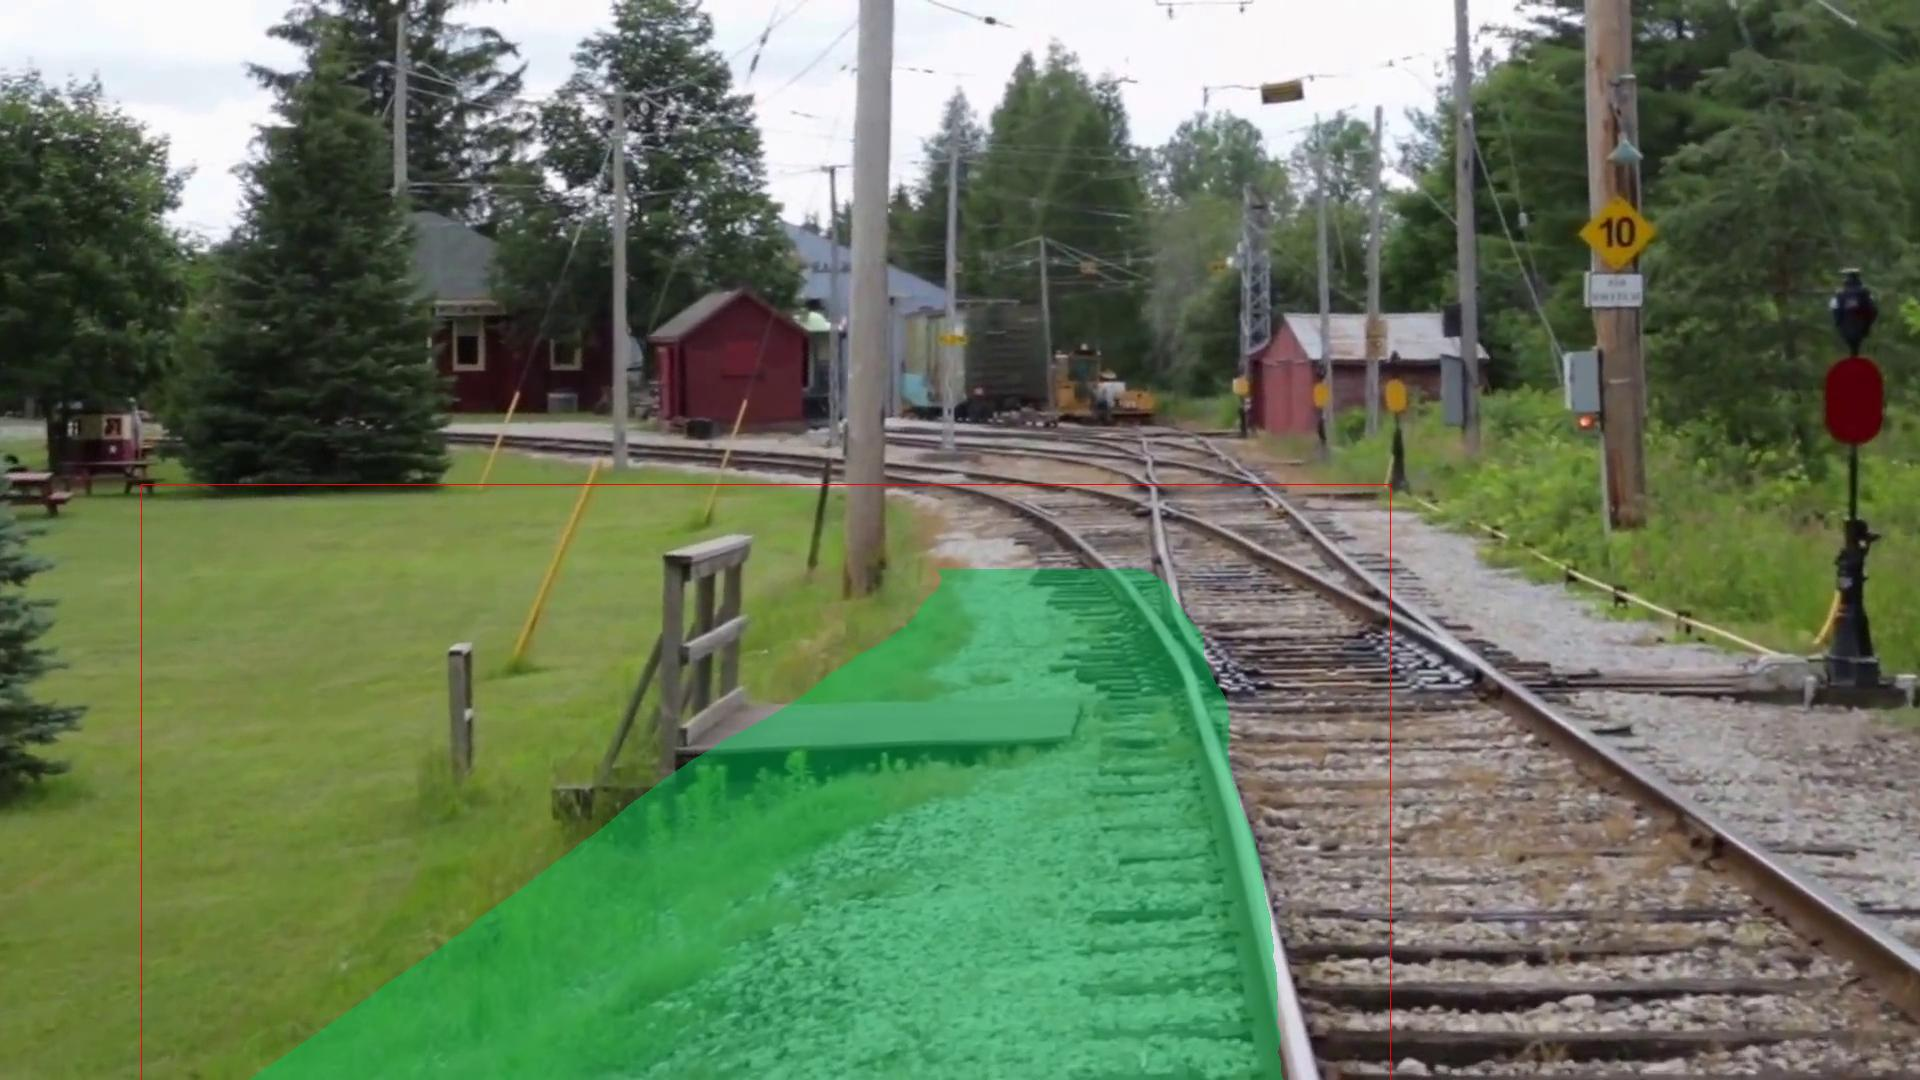
\includegraphics[width=\textwidth]{PICs/experiments/ComparisonBaselineToImproved/original2.jpg}
        \end{subfigure}
        \begin{subfigure}[b]{0.48\textwidth}
            \centering
            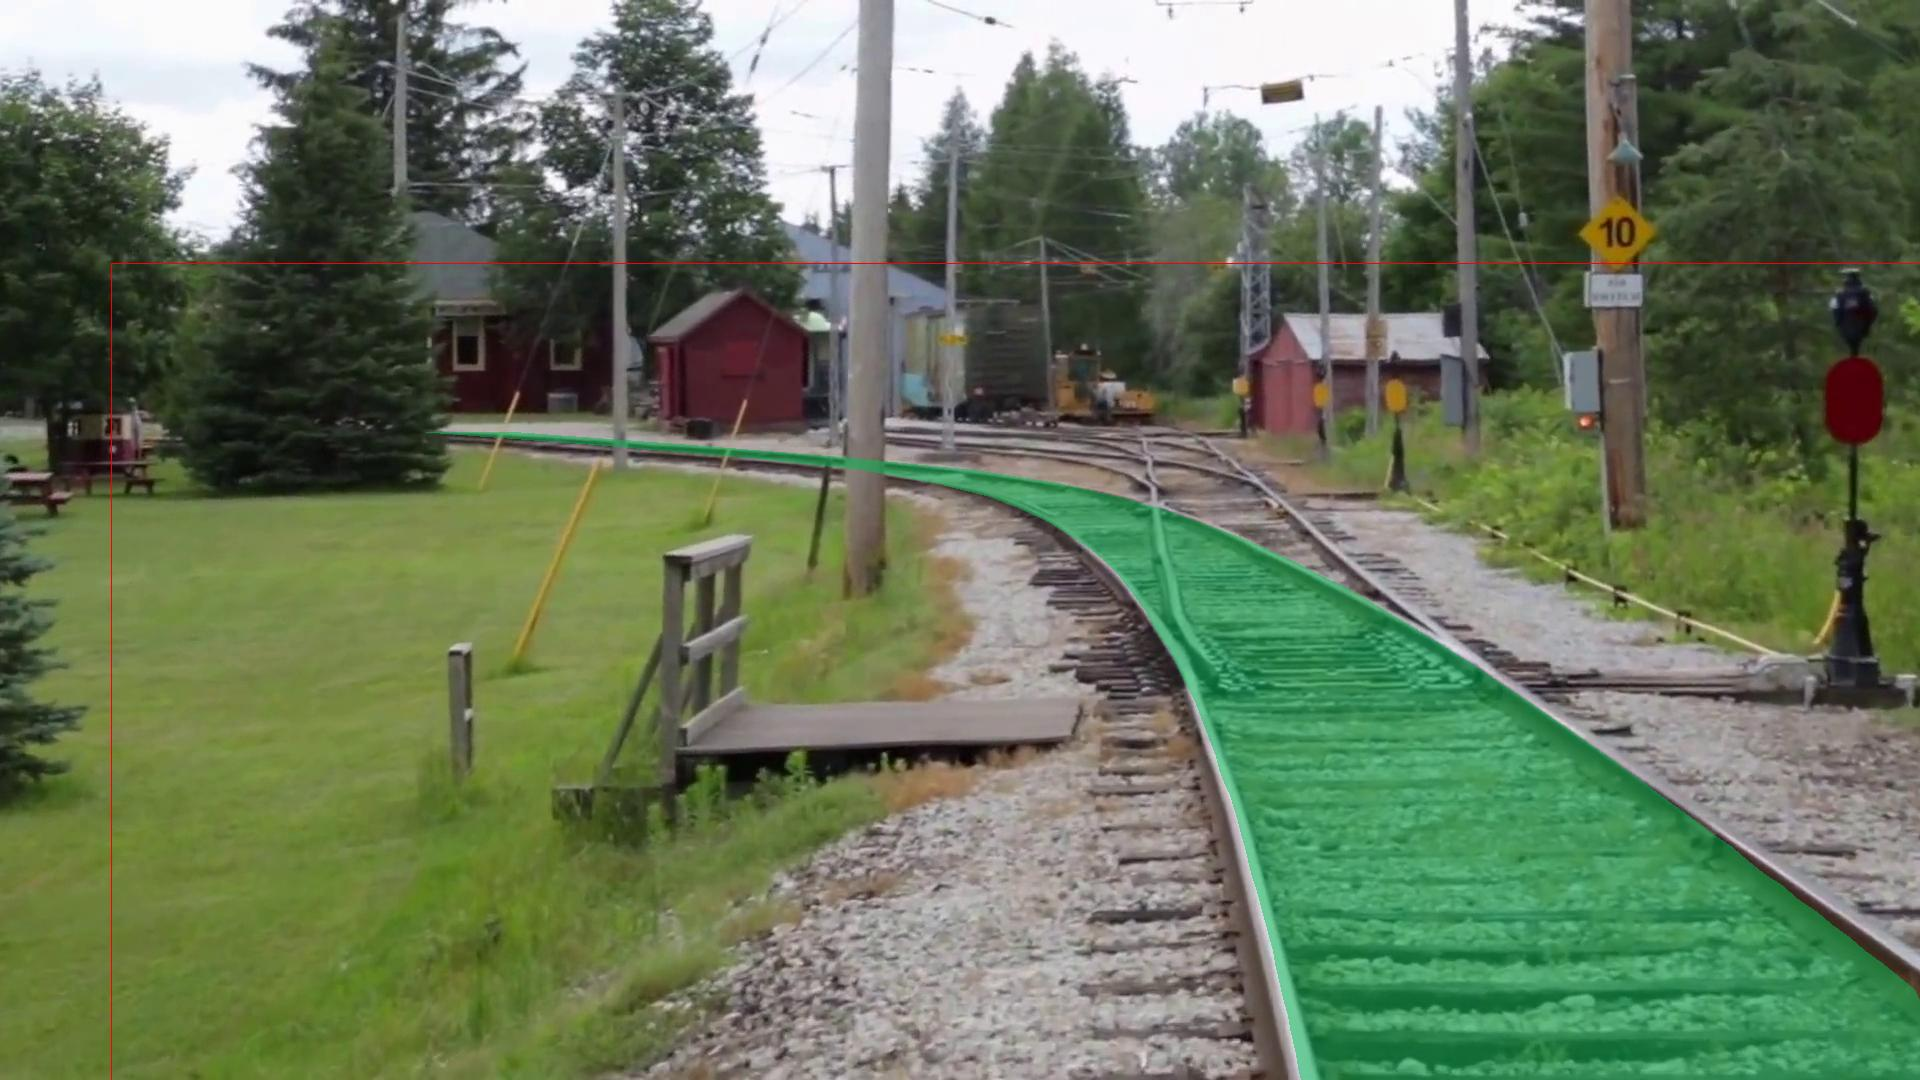
\includegraphics[width=\textwidth]{PICs/experiments/ComparisonBaselineToImproved/adapted2.jpg}
        \end{subfigure}
        
        \vspace{0.5cm} % Abstand zwischen den Zeilen
        
        \begin{subfigure}[b]{0.48\textwidth}
            \centering
            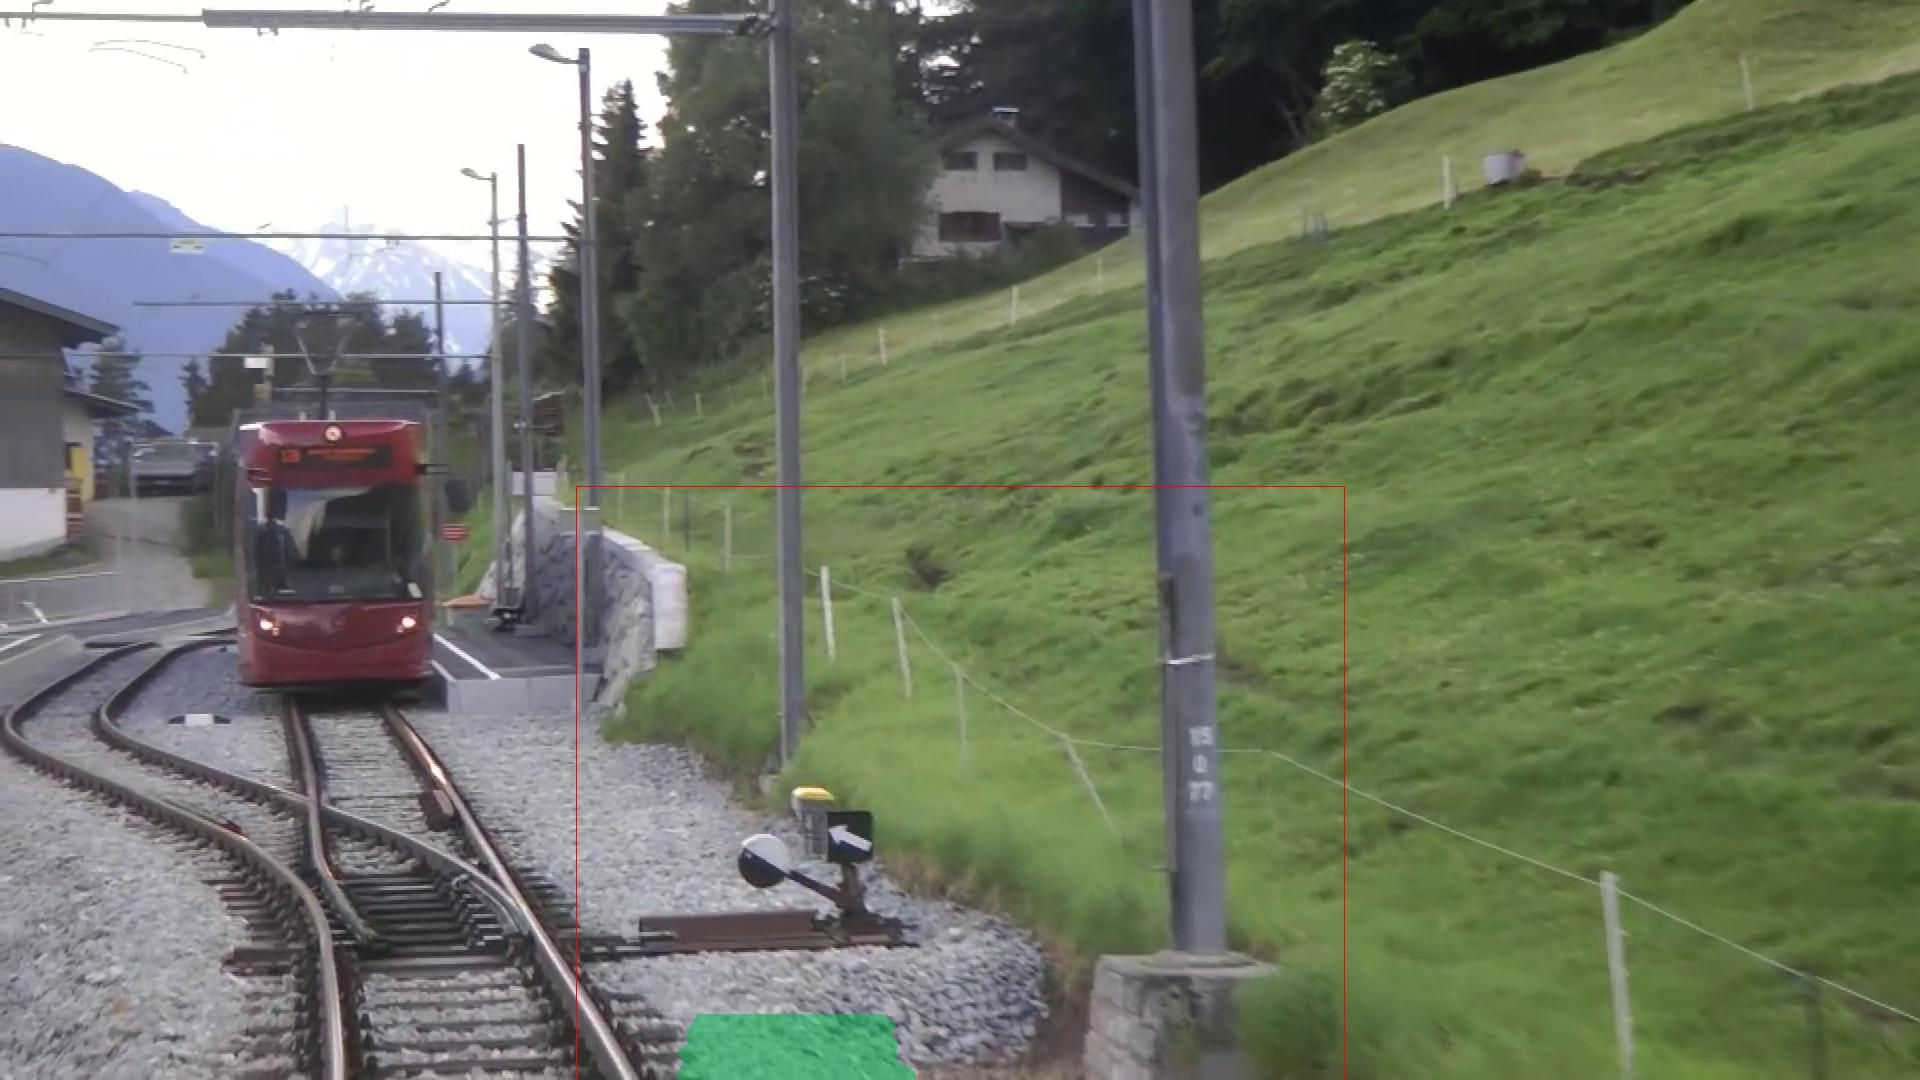
\includegraphics[width=\textwidth]{PICs/experiments/ComparisonBaselineToImproved/original1.jpg}
        \end{subfigure}
        \begin{subfigure}[b]{0.48\textwidth}
            \centering
            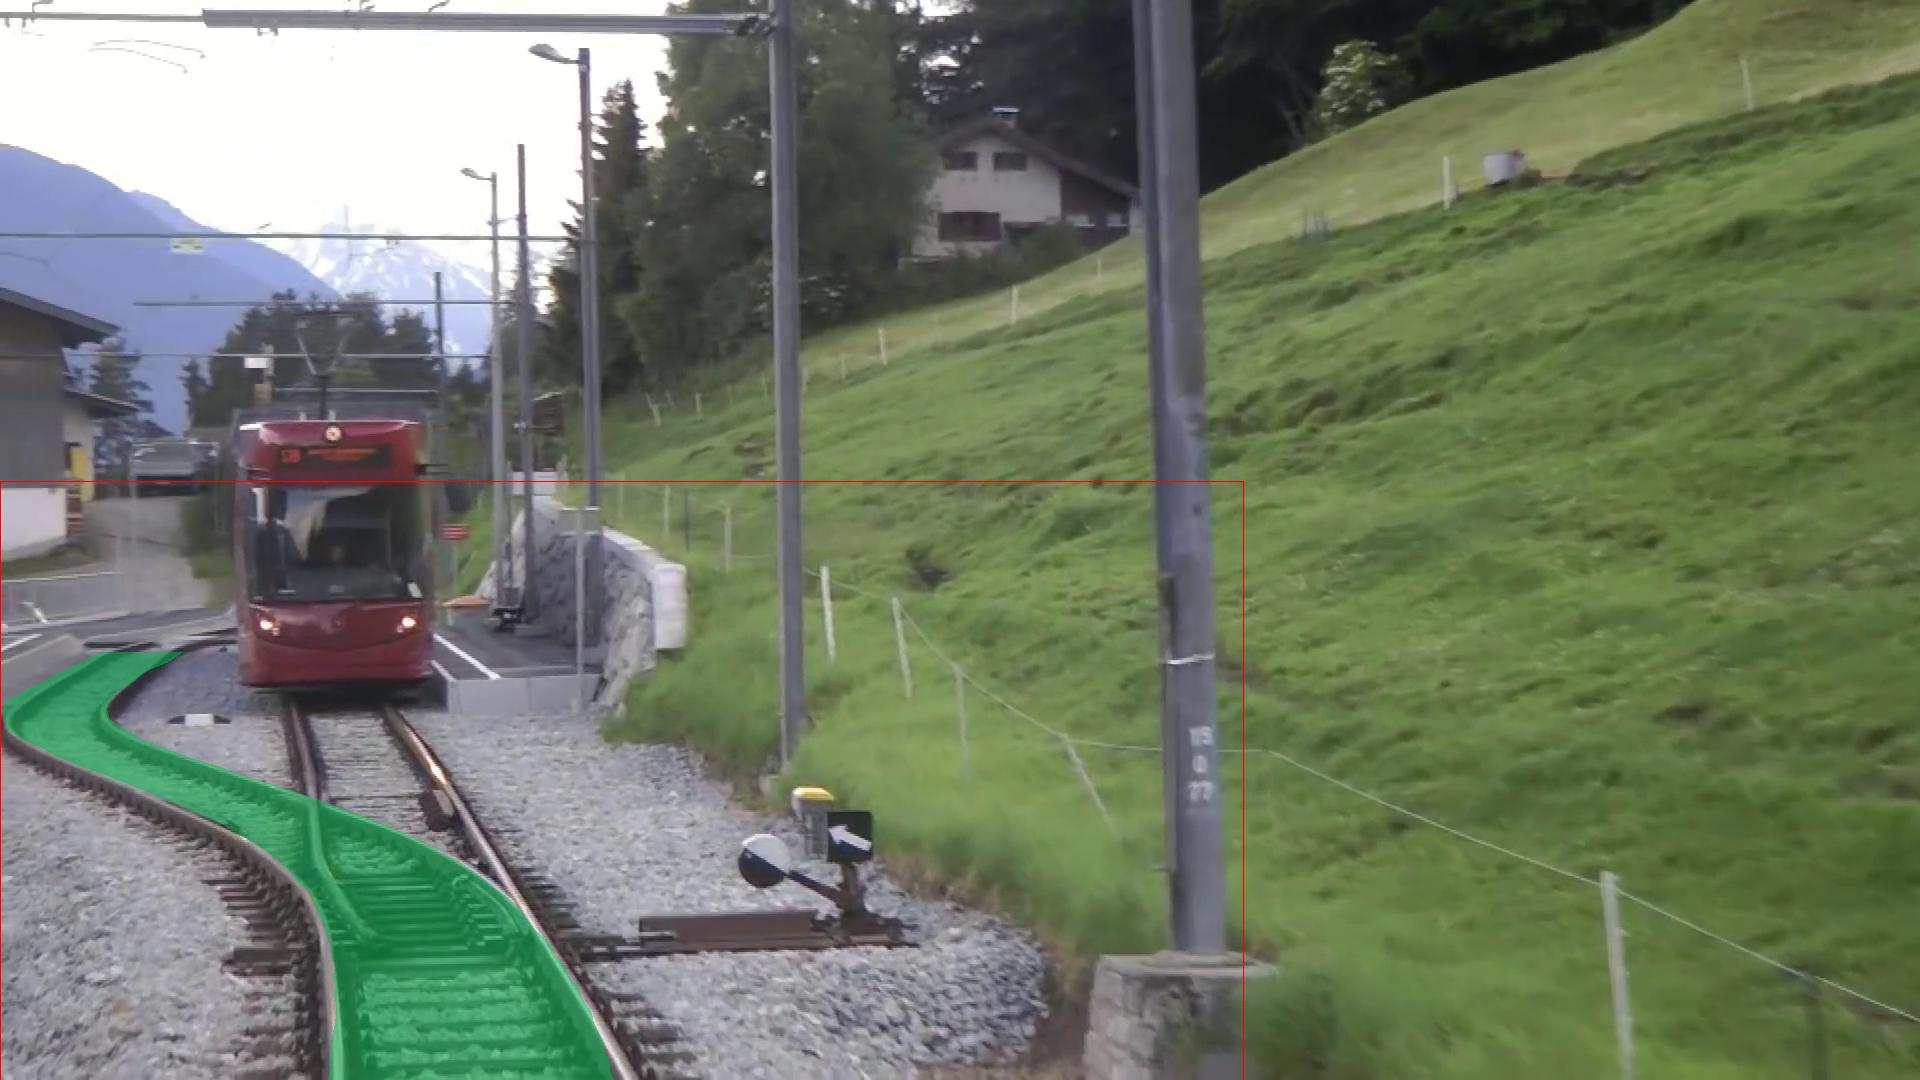
\includegraphics[width=\textwidth]{PICs/experiments/ComparisonBaselineToImproved/adapted1.jpg}
        \end{subfigure}
        
        \vspace{0.5cm} % Abstand zwischen den Zeilen
        
        \begin{subfigure}[b]{0.48\textwidth}
            \centering
            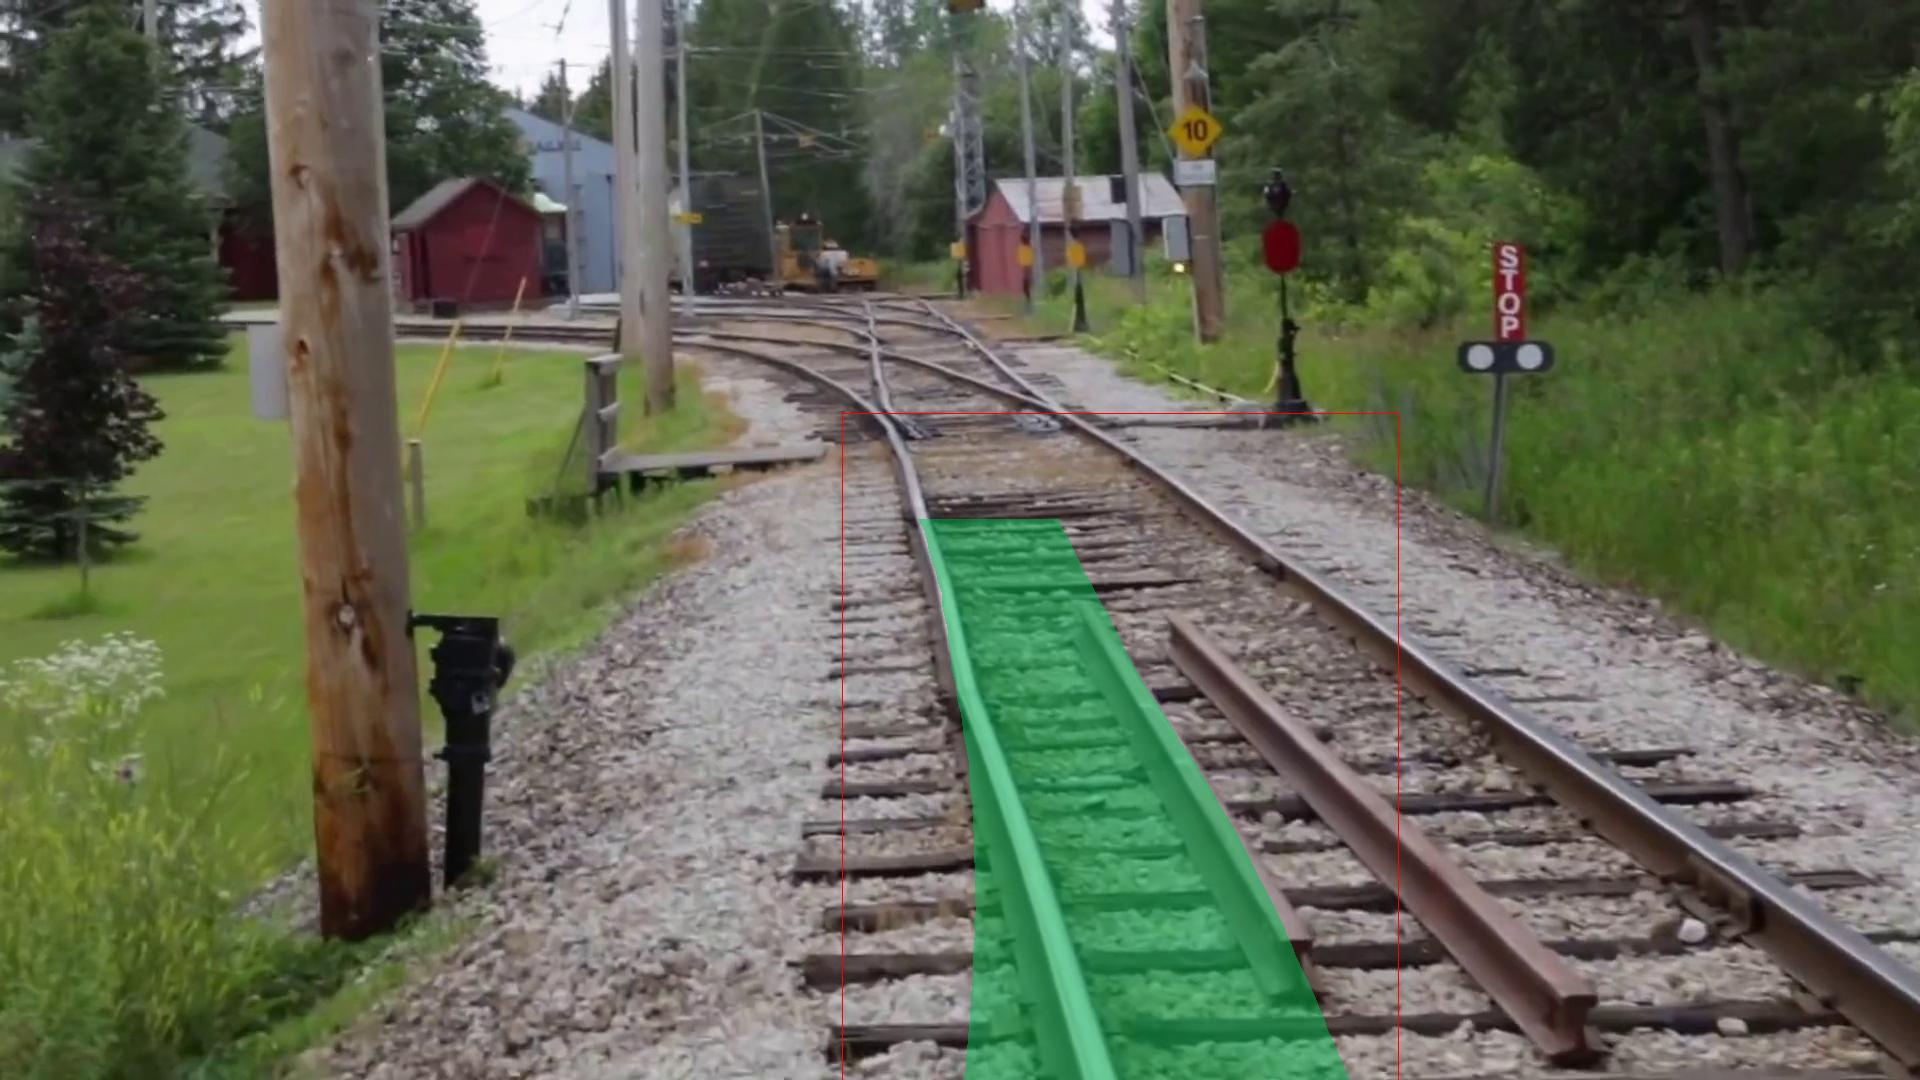
\includegraphics[width=\textwidth]{PICs/experiments/ComparisonBaselineToImproved/original3.jpg}
        \end{subfigure}
        \begin{subfigure}[b]{0.48\textwidth}
            \centering
            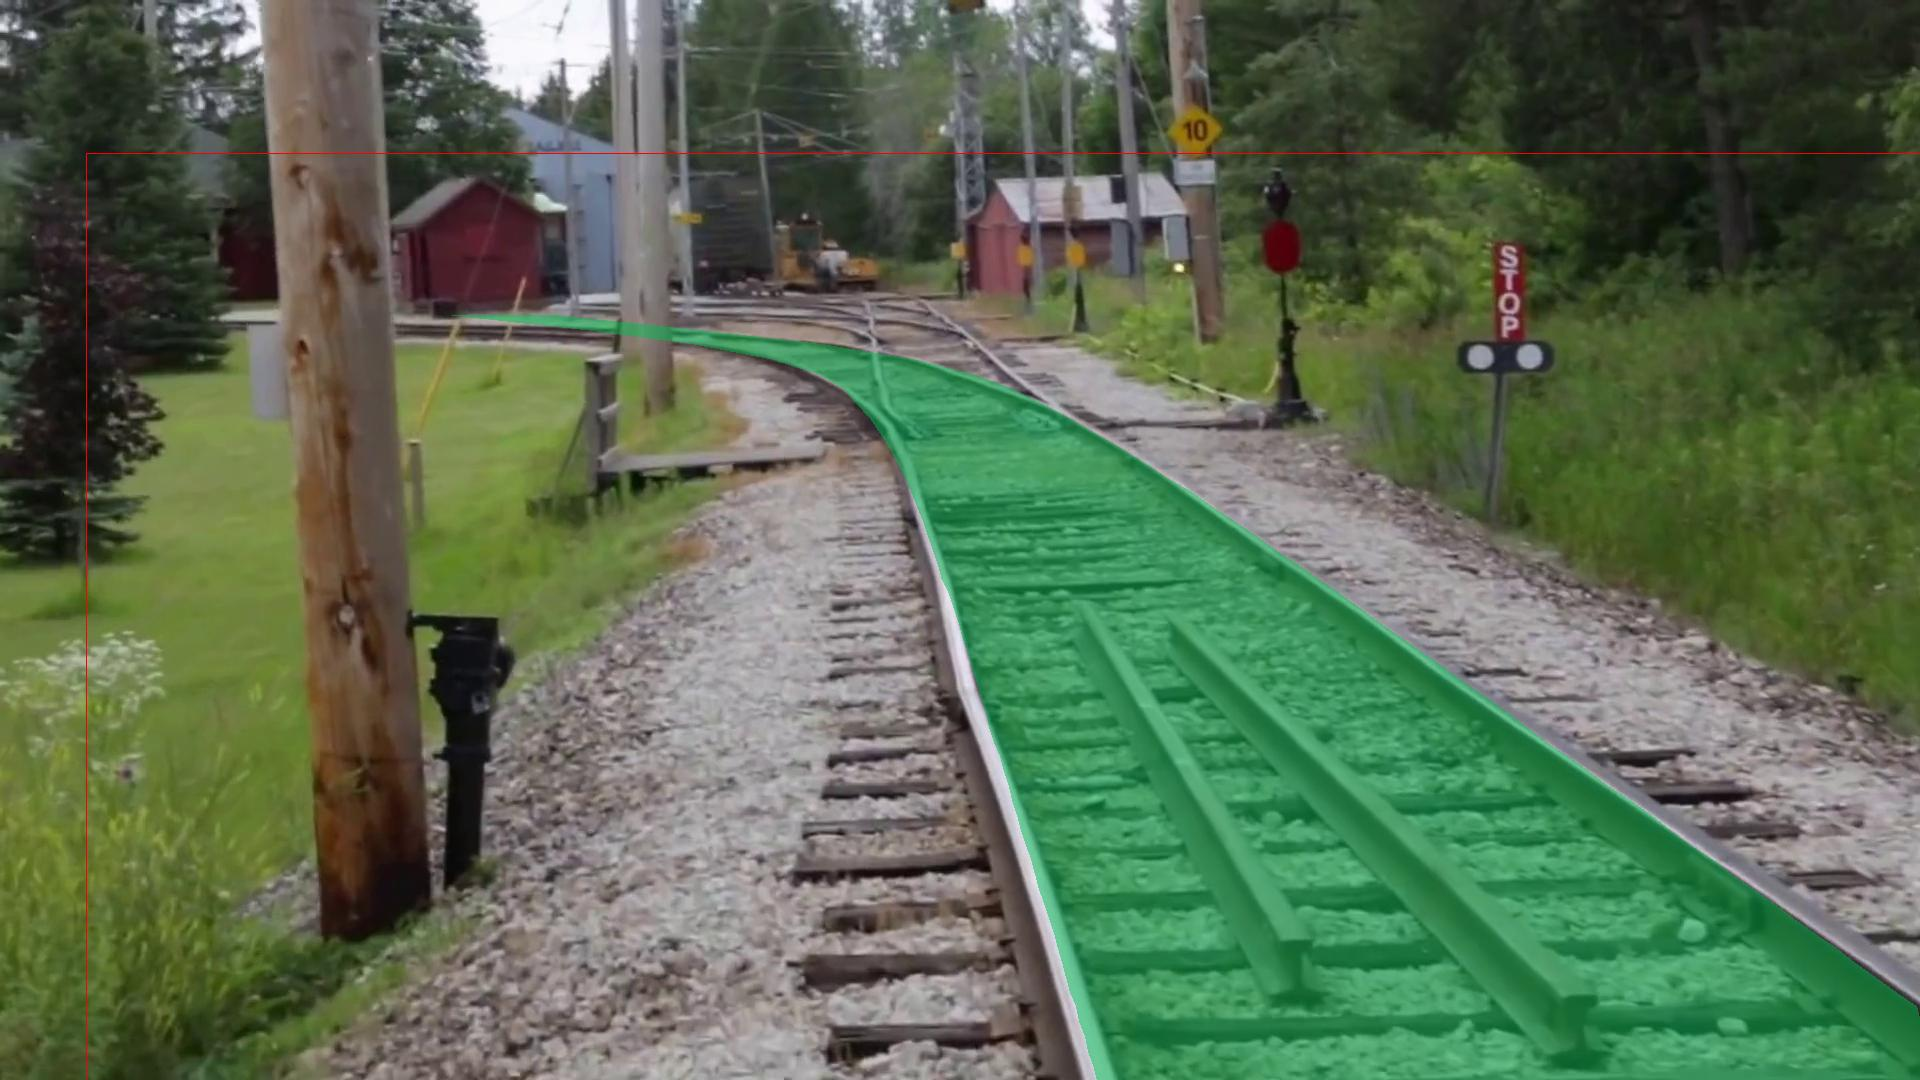
\includegraphics[width=\textwidth]{PICs/experiments/ComparisonBaselineToImproved/adapted3.jpg}
        \end{subfigure}
    \end{minipage}%
    \hfill
    \begin{minipage}{0.2\textwidth} % Rechte Seite für Text
        \centering
        \textbf{adapted TEP-Net}\\
        EfficientNet-B3
    \end{minipage}
    \caption{Comparison between the best version of TEP-Net \cite{tepNet2024} and the best version with all improvements of this work: best backbone, adaptive max pooling, trapeze head and adapted auto-crop mechanism.
    Images of complex scenes with difficult angles of perspective are intenionally chosen.}
    \label{fig:comparisonBaseline2Improved}
\end{figure}